\section{Implementierung der Simulation und des Experiments}

Fortfolgend an die in der letzten Sektion beschriebenen Anforderungen, wird in dieser Sektion die finale Implementierung der einzelnen Programmabschnitte erläutert.
In Anlehnung an den Aufbau der letzten Sektion, wird die Umsetzung der Anforderungen zu den Programmabschnitten Simulationsumgebung, Trainingsverfahrens und Laborexperiment dargelegt.

Allgemeiner Natur ist die Wahl der Entwicklungssprache Python.
Die Entwicklungssprache ermöglicht eine hohe Kompatibilität mit bekannten Simulationsframeworks, RL-Softwarebibliotheken und Bibliotheken zur statischen Auswertung von Messdaten.
Im Rahmen dieser Arbeit wird konkret die Python Version 3.10 eingesetzt, um von den Möglichkeiten neuer Funktionen zu profitieren und zugleich eine möglichst hohe Kompatibilität zu existieren frei verfügbaren Bibliotheken aufzuweisen.
Alle in dieser Arbeit verwendeten Bibliotheken sowie deren Abhängigkeiten sind in einer virtuellen Umgebung installiert, sodass bestmöglich Störeinflüsse durch bereits installierte Pakete vermieden werden.
Ebenso sind alle eingesetzten Softwarepakete in einer Textdatei inklusive ihrer Version dokumentiert.

\subsection{Programmumsetzung der Simulationsumgebung}

Die Umsetzung der Anforderungen der Simulationsumgebung beinhaltet im Fokus die Entwicklung einer Simulationsumgebung anhand des Gymnasium Programmiergerüsts.
Die entwickelte Simulation baut dabei auf bestehende Programmbibliotheken auf.
Dies fördert vor allem die im Zuge dieser Arbeit umsetzbare Qualität und ermöglicht einen hohen Grad an Realismus, welcher wie in den Anforderungen beschrieben unmittelbar das Sim2Real Problem und damit die Robustheit beeinflusst.
Weiterhin stellt die Neuentwicklung einer Simulationsumgebung kein Entwicklungsaufwand dar, welcher einen Einfluss auf die auszuwertende Forschungsfrage ausübt.
Wird die im zweiten Kapitel angeführte Auswahl an in der Literatur beschriebenen Simulationsumgebungen betrachtet, kann aus diesen eine Basis zur Entwicklung der eigenen Simulationen gewählt werden.

% Beschreibung der Auswahlkriterien
Zur Auswahl einer Basissimulation, in welcher die eigenen Trainings- und Testszenarien abgebildet werden können, sind unterschiedliche Kriterien zu beachten.
Ein Kriterium ist die Kompatibilität der Basissimulation mit der gewählten Entwicklungssprache. 
Hierbei sollte entweder die Simulation selbst in Python, oder eine entsprechende Schnittstelle entwickelt sein.
Die gewählte Simulation sollte eine Physik-Engine einsetzen, welche zum einen einen möglichst hohen Grad an Realismus erlaubt, um die Forschungsfrage möglichst valide zu beantworten.
Zum Anderen sollte die Simulation einen beherrschbaren Rechenleistungsaufwand verursachen, da die Zielsetzung die Optimierung mehrerer Policies beinhaltet.
Weiterhin, zur Erfüllung der zuvor beschriebenen Anforderungen, muss die Basissimulation dem Framework Gym oder dessen Nachfolger Gymnasium entsprechen.
Um die Entwicklung des Optimierungsverfahrens zu unterstützen wird eine RL Integration oder zumindest eine Umfangreiche Dokumentation zu dessen Einsatz vorausgesetzt.
Die nachfolgende Tabelle stellt die in Betracht gezogenen Drohnensimulationen den für die Auswahl getroffenen Kriterien gegenüber.

\begin{table}[H]
    \centering
    \begin{tabular}{l|l|l|l|l|}
    \cline{2-5}
                                         & RotorS & CrazyS & AirSim & gym-pybullet-drones \\ \hline
    \multicolumn{1}{|l|}{Python API}     &   X    &   X    &   X     &       X             \\ \hline
    \multicolumn{1}{|l|}{\begin{tabular}[c]{@{}l@{}}Integration des \\ Gymnasium Frameworks\end{tabular}} & X & X & X & X \\ \hline
    \multicolumn{1}{|l|}{höchster Realismusgrad} &        &        &    X    &                 \\ \hline
    \multicolumn{1}{|l|}{\begin{tabular}[c]{@{}l@{}}kontrollierbarer \\ Rechenleistungsaufwand\end{tabular}} &    X    &    X    &      &     X\\ \hline
    \multicolumn{1}{|l|}{\begin{tabular}[c]{@{}l@{}}umfangreiche \\ RL Integration \\ und Dokumentation\end{tabular}}           &  &  & X & X \\ \hline
    \multicolumn{1}{|l|}{\begin{tabular}[c]{@{}l@{}}Simulation mehrerer\\ Quadrokopter \\ enthalten \end{tabular}}           &  &  &  & X \\ \hline
    \end{tabular}
    \caption{Gegenüberstellung von Auswahlkriterien und bekannten Drohnensimulationen}
    \label{tab:drone-simulation}
\end{table}
\footnotetext{Eigene Darstellung}

Aus der Gegenüberstellung von Auswahlkriterien und aktuellen Simulation geht hervor, dass zunächst alle Simulationen eine Schnittstelle für die Entwicklungssprache bereitstellen.
Dabei wurden native Schnittstellen sowie Schnittstellen aus zusätzlichen Softwarebibliotheken miteinbezogen.
Auch die Integration des Gym oder Gymnasium Frameworks wird durch alle Simulationen eigens oder durch zusätzliche Bibliotheken sichergestellt.
Bei der Betrachtung der Realitätsnähe zeigt die AirSim Umgebung aufgrund der verwendeten Unreal Physik-Engine den höchsten Grad an Realismus auf.
Im Gegenzug werden durch diese Simulation Rechenkapazitäten erwartet, welche im Rahmen dieser Arbeit nicht zur Verfügung stehen.
Eine umfangreiche Dokumentation und bereits vorhandene Integration von RL wird durch AirSim und gym-pybullet-drones gewährleistet.
Die Simulationen RotorS und CrazyS bieten eine Integration mit RL nur auf Basis der wenig dokumentierten zusätzlichen Softwarebibliotheken GymFC und gym\_multirotor.
Wird das letzte Kriterium der Simulation mehrerer Drohnen betrachtet, tritt dies nur in Beispielen der gym-pybullet-drones Simulation auf.
%Fazit
Fasst man die Erfüllung der Auswahlkriterien zusammen wird erkenntlich, dass gym-pybullet-drones als einzige Drohnensimulationen die zusätzlichen Anforderungen der RL Integration und der Dokumentation erfüllt.
Demnach wird für die nachfolgende Entwicklung der eigenen Simulation auf der gym-pybullet-drones Bibliothek aufgebaut.

Die gym-pybullet-drones Simulation ist in einzelne Simulationszenarien gegliedert, welche je eine Python Datei umfassen.
Als Aviaries gekennzeichnet, bilden sie je eine Trainingsumgebung nach der Schnittstellendefinition des Gymnasium Frameworks ab.
In der Struktur der Simulationsumgebung wird das Programmierkonzept der Vererbung verwendet, um ähnliche Simulationen auf den selben übergeordneten Klassen zu basieren.
Jede erbende Klasse enthält damit alle Funktionen und Variablen der übergeordneten Elternklasse.
Dies ermöglicht die verschieden starke Abstraktion der Simulation auf den unterschiedlichen Vererbungsebenen.
Weiterhin ermöglicht die Bibliothek verschiedene Steuerungsarten der Quadrokopter. 
Eine Option ist die Steuerung über die direkte Vorgabe der Drehzahlen aller Rotatoren. 
Zusätzlich kann auch ein PID-Kontroller eingesetzt werden um die Steuerungssignale entgegenzunehmen.
Zur Entwicklung der eigenen Simulation wird die Steuerung über einen Richtungsvektor und einen Geschwindigkeitswert gewählt.
Unabhängig des gewählten Aktionstyps werden alle Steuerungssignale durch Controllerklassen in konkrete Drehzahlen übersetzt.
Dessen genaue Übersetzung wird im Rahmen dieses Kapitels nicht erläutert und ist in der entsprechenden Dokumentation nach \cite[]{Panerati.332021} nachzulesen.
Auch der Beobachtungsraum kann zum einen visuell und zum anderen kinetisch erfolgen, was im Rahmen dieser Arbeit verwendet wird.
Der kinetische Beobachtungsraum stellt eine Reihe von wahrnehmbaren Eigenschaften wie Position, Ausrichtung, Geschwindigkeit und Drehzahl dar.
Unabhängig der Überwachungsart wird durch die pybullet Physik-Engine ein grafisches Modell der Simulation erzeugt.
Unter visuellem Beobachtungsraum wird dieses durch eine Drohnenkamera als Sammlung aller Pixelwerte eines 64x48 großen Bildes wahrgenommen.
%Die nachfolgenden Abbildungen zeigen die grafische Simulation und den visuellen Beobachtungsraum.

% Grundbasis der eigenen Simulation
Die Umsetzung, der zu Beginn dieses Kapitels beschriebenen Simulationsumgebung, basiert auf der Verwendung der Basissimulation und der Kontrollerklassen. 
Zusätzlich sind teilweise Funktionen aus ähnlichen bereits nativ vorhandenen Szenarien mit Änderungen übernommen und im Programm entsprechend gekennzeichnet.
Die beschriebene Simulation ist innerhalb einer Klasse nach dem Gymnasium Framework aufgebaut.
Zusätzlich wird die Simulation durch eine erbende Klasse umhüllt, um für den Algorithmus eine verarbeitbare Abstraktionsschicht zu erzeugen.
In dieser Schicht wird die Steuerung der angreifenden Drohne abstrahiert, sodass die Trainingsumgebung lediglich die Bestimmung einer Aktion für die verteidigende Drohne erwartet.
Nachfolgend wird die Umsetzung dieser beiden Klassen nach den einzelnen Funktionen des Gymnasium Frameworks erläutert.

% Init DualDrone Aviary
Die Simulation beider Quadrokopter ist in der Klasse \textbf{DualDroneAviary} definiert.
Zur Initialisierung einer Simulationsinstanz wird die \textbf{Init-Funktion} aufgerufen, welche die Übergabe aller simulations relevanten Parameter erwartet.
Die Parameter umfassen unter anderem Informationen zur Anzahl und Art und Position der Drohnen, gewählte Handlungs- und Beobachtungsarten sowie die unabhängigen Variablen der Trainingsszenarien.
Außerdem wird die Gewichtung der Belohnungsfunktion als Parameter entgegen genommen.
Kernaufgabe dieser Funktion ist die Umsetzung der Eigenschaften eines Trainings- und Testszenarios.
Dies beinhaltet die Erzeugung und Übermittlung der zufälligen Start- und Zielpunkte und des zufälligen Windeffektes mittels unterstützender Funktionen aus der eigenen Hilfsklasse.
Sind die Eigenschaften bestimmt, können diese zur Erzeugung der darunter liegenden Abstraktionsschicht der BaseAviary Instanz genutzt werden.

% Observation Space
Der \textbf{Beobachtungsraum} in dieser Simulation wird durch einen Informationsvektor definiert.
Der für die Experimente eingesetzte Informationsvektor je Drohne enthält die Position, Ausrichtung, Fortbewegungs- und Drehgeschwindigkeit sowie die Rotationsdrehzahlen.
Die Position ist durch die dreidimensionale Koordinaten, die Ausrichtung durch Quaternion und Drehwinkel kodiert.
Positionen können dabei von $- \inf$ bis $+ \inf$ in X- und Y-Richtung und von $0$ bis $+ \inf$ in Z-Richtung betrachtet werden.
Die Quaternion erlauben Werte zwischen $-1$ und $+1$, die Drehwinkel von $- \pi$ bis $+ \pi$
Drohnen-, Dreh-, und Rotatorengeschwindigkeit werden als Geschwindigkeitsvektor von minus bis plus unendlich zu den Koordinatenachsen bzw. als vier einzelne Werte von Null bis zu maximalen Drehzahl definiert.
Insgesamt ist für jede Drohne ein Beobachtungsvektor mit 20 Elementen innerhalb eines Wörterbuchobjektes definiert.

% Action Space
Die Definition des \textbf{Aktionsraums} ist in der ActionSpace Funktion bestimmt.
Je nach Aktionstyp ist ein drei oder vierdimensionaler Vektorbereich definiert.
Jeder Wert des Vektors kann besitzt eine untere und obere Grenze aus dessen Bereich die endgültige Aktion gewählt wird.
Zur Steuerung des Quadrokopters wird im Rahmen dieser Arbeit der Aktionstyp auf Basis der Geschwindigkeit verwendet.
Der Wertebereich des Richtungsvektors ist dabei von $[-1,-1,-1]$ bis $[1,1,1]$ definiert. 
Das vierte Element spiegelt den Anteil der maximalen Geschwindigkeit von null bis eins wieder.

% Step 
Ist eine Aktion regelbasiert oder durch einen RL-Modell bestimmt, wird diese als Parameter an die \textbf{Step-Funktion} weitergegeben.
Auf der Ebene der DualDroneAviary Klasse kann die übergebene Aktion in Abhängigkeit vom anfangs initialisierten Wind abgewandelt werden.
Der Windvektor wird in Abhängigkeit des Winkels zwischen Bewegungsrichtung der Drohne und des Windes zur Aktion hinzugefügt.
Der Drohnenbewegungsrichtung wird die Windrichtung addiert und die Geschwindigkeit in Abhängigkeit des Eintreffwinkels vollständig postiv, negativ oder gar nicht beeinflusst.
Anschließend wird unter veränderter oder unveränderter Aktion die Schrittfunktion der Elternklasse aufgerufen.
Die Schrittfunktion der Elternklasse übersetzt die Aktion aus dem Aktionsraum in konkrete Rotorendrehzahlen und übt diese unter der simulierten Physik aus.
Zur Erhöhung des Realismusgrads wird zusätzlich zu den Effekten der pybullet Physik-Engine ein Boden- und Trägheitseffekt eingesetzt.
Anschließend wird die neue Zustandsbeobachtung, die entstandene Belohnung, das Rücksetzkriterium und ein Datenobjekt für Zusatzinformationen zurückgegeben.

% Reward ?
Die Bestimmung des Rewards ist unter der \textbf{reward-Funktion} der DualDroneAviary Klasse implementiert.
Innerhalb dieser Funktion werden aus dem aktuellen Zustand der Simulation Kennzahlen zu dessen Evaluation berechnet und gewichtet.
Durch die Gewichtung und dessen Optimierung kann das Strategieziel formuliert und der Einfluss des Wertebereichs der Kennzahlen angepasst werden.
Die Aufsummierung der Produkte aus den folgenden Kennzahlen und deren Gewichtung spiegelt die Belohnung zu jedem Zeitschritt wieder.
\begin{itemize}
    \item Distanz zwischen der angreifenden und verteidigenden Drohne
    \item Belohnung bei erfolgreichem Abfangen der angreifenden Drohne
    \item negative Belohnung sofern der Zielpunkt erreicht wurde
    \item Belohnung für eine möglichst direkte Flugrichtung zur gegnerischen Drohne
    \item Lineare Belohnung der Geschwindigkeit
\end{itemize}
Eine Optimierung der Gewichte wurde durch Ausprobieren unterschiedlicher Gewichtskombinationen und Messen der entsprechenden Erfolgsrate erzielt.
Zu jedem Zeitschritt eintretende Kennzahlen wurden aufgrund ihrer Häufigkeit in Fünfer Schritten, außerordentliche Belohnungen in 10000er Schritten untersucht.
Insgesamt sind daraus folgende Log-Dateien entstanden, welche den Optimierungsprozess wiederspiegeln.

\begin{figure}[htb]
    \centering
    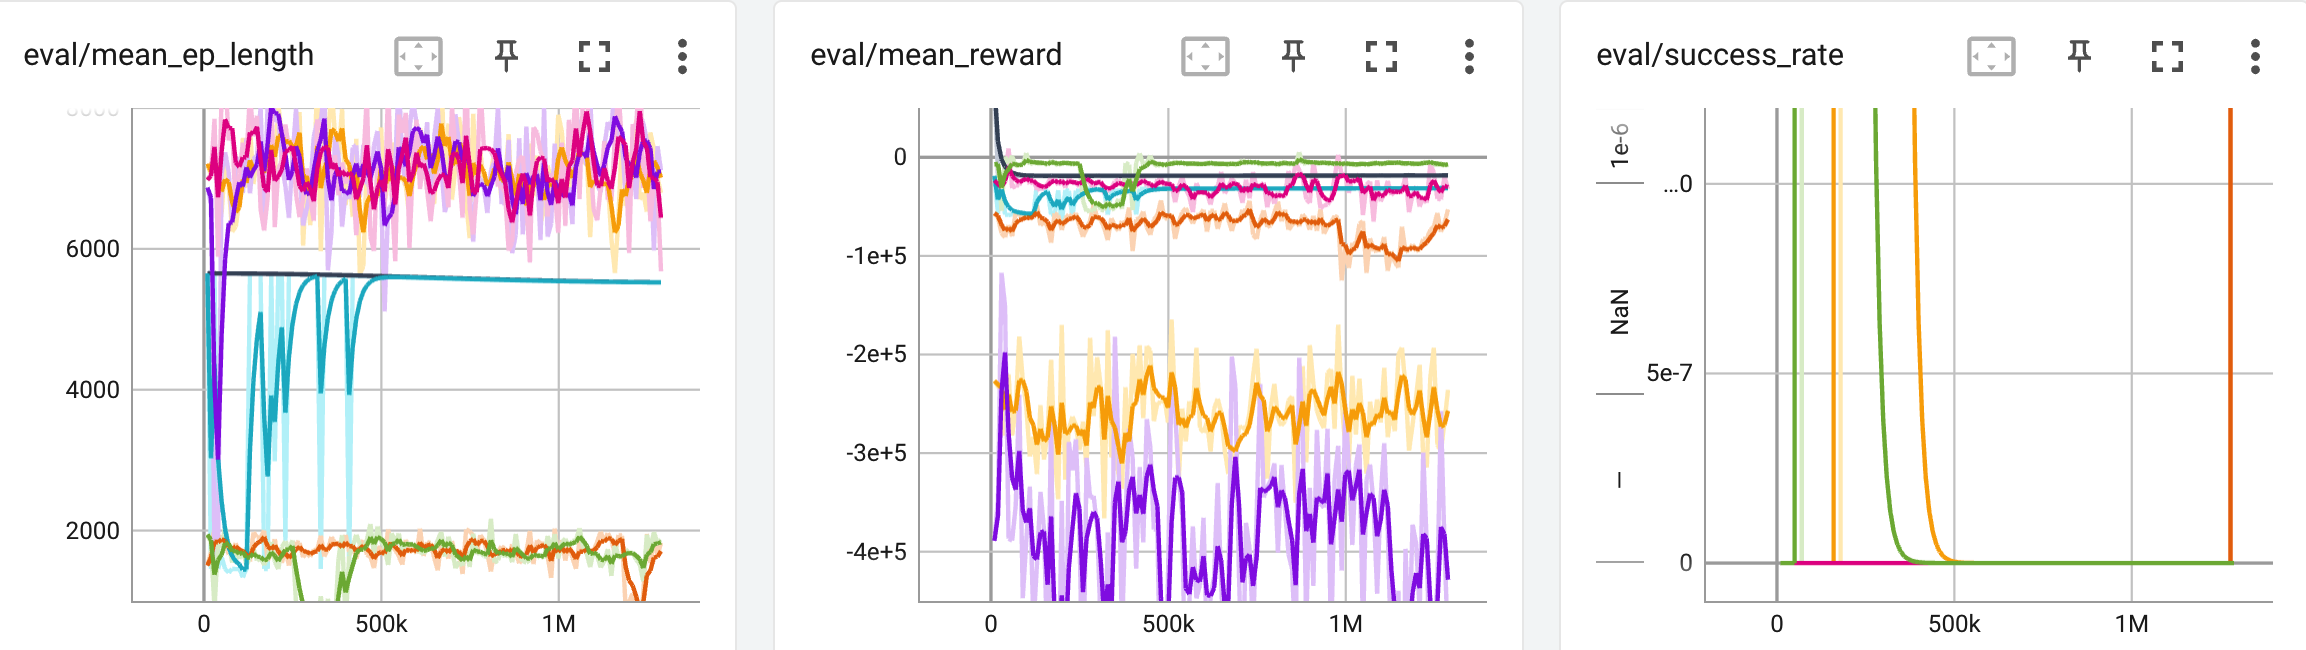
\includegraphics[height=4.5cm]{lib/graphics/speed_reward_logs.png}
    \caption[Episodenlänge, Belohnung und Erfolgsrate unter verschiedenen Gewichtungen]{Episodenlänge, Belohnung und Erfolgsrate unter verschiedenen Gewichtungen\footnotemark}
    \label{abb:reward-logs}
\end{figure}
\footnotetext{Darstellung der Tensorboarddaten}

Die Optimierung der Belohnungsfunktion brachte $[-10, 50000, 50000, 25, 20]$ als optimalen Gewichtsvektor hervor, da hierunter mehrere Algorithmen wie PPO und A2C, eine positive Erfolgsrate verzeichneten.

% reset
Ist das Rücksetzkriterium erfüllt wird die Simulationsumgebung mittels \textbf{reset-Funktion} neugestartet.
Dabei sind neue Zufallspositionen der Drohnen und des Ziels sowie im vierten Trainingsszenario eine neue Windeigenschaften zu generieren.
Sind diese Variablen verändert kann die Rücksetzfunktion der darunterliegenden Abstraktionsschicht aufgerufen werden.
Die Funktion der BaseAviary-Klasse setzt darin die Zeitschritte und die Drohneninformationen zurück und baut das grafische Modell neu auf.
Über den Zugriff auf den Klienten der pybullet Physik-Engine werden die Drohnenobjekte sowie das Untergrundobjekt aus den URDF-Dateien geladen und an entsprechenden Stellen platziert.
Zur Unterscheidung des verteidigenden Quadrokopters von der angreifenden Drohne werden zwei nahezu identische URDF-Dateien verwendet, welche sich nur in der Farbgebung zwischen rot und blau unterscheiden.
Am Ende der Funktion wird der erste Beobachtungsvektor der neuen Episode sowie ein Infoobjekt zurückgegeben.

% Single Drone Wrapper
Die zuvor beschriebene Klasse vererbt ihre Variablen und Funktionen auf die höhergelegene Abstraktionsschicht der \textbf{SingleDroneWrapper} Klasse.
Auf dieser Ebene wird bietet die Simulation ihre Schnittstelle für die Verwendung durch den IL- und RL-Algorithmus.
Dafür ist es notwendig den Beobachtungsraum sowie den Aktionsraum zu neu zu definieren.

Zur \textbf{Initialisierung} werden zum einen alle Parameter zur Instanziierung des DualDroneAviary Objekt erwartet.
Zum Anderen sind zusätzlich die Strategie und dessen Rauschverhalten der angreifenden Drohne anzugeben, sodass diese in Klassenvariablen gespeichert werden.
Auf der Ebene des SingleDroneWrapper-Klasse wird der \textbf{Beobachtungsraum} mit allen Informationen beider Quadrokopter zu einem 40-elementigen Vektor zusammengefasst.
Der \textbf{Handlungsraum} hingegen umfasst auf dieser Ebene lediglich einen elementigen Vektor mit dem bekannten Wertebereich.
Zur Ausführung eines Simulationsschrittes werden in der \textbf{Step-Funtkion} die Aktion der Angreiferstrategie und die übergebene Aktion in ein Datenobjekt überführt.
Anschließend kann mittels diesen Datenobjektes die Schrittfunktion der Elternklasse aufgerufen, und deren Rückgabewerte an den zu optimierenden Algorithmus weitergereicht werden.
Als \textbf{Belohnungswert} wird dabei lediglich auf die im Trainingsszenario relevante Kompontente des Belohnungsobjektes zugegriffen.

Fasst man die beschriebene Umsetzung der Simulationsumgebung zusammen, so kann folgendes Klassendiagramm und deren Funktionsabhängigkeiten in Abbildung Acht betrachtet werden.

\begin{figure}[htb]
    \centering
    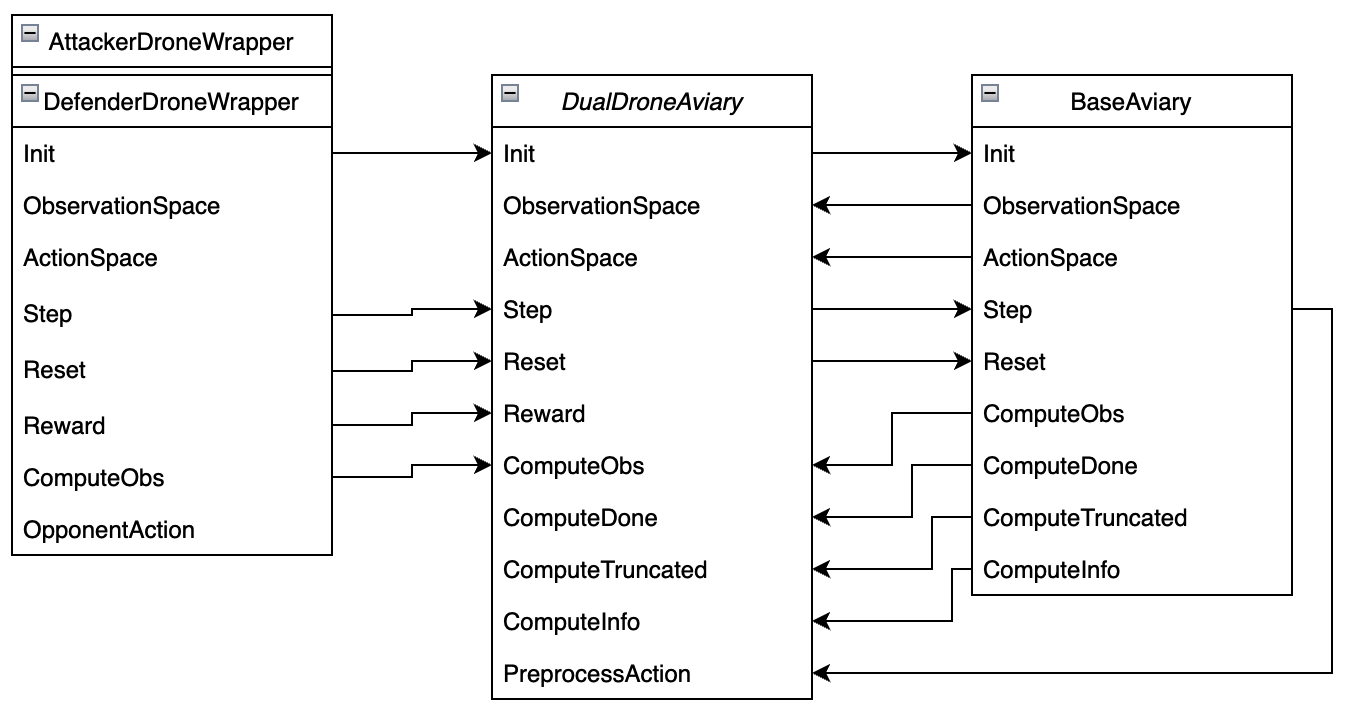
\includegraphics[height=6cm]{lib/graphics/simenv structure.png}
    \caption[Klassendiagramm mit Funktionabhängigkeiten]{Klassendiagramm mit Funktionabhängigkeiten\footnotemark}
    \label{abb:drone axis}
\end{figure}
\footnotetext{Eigene Darstellung}

\subsection{Programmumsetzung des Optimierungsverfahrens}

Mit der Entwicklung der Simulationsumgebung stehen Trainingsdaten zur Verfügung darauf aufbauend Strategien des verstärkenden Lernens zu optimieren.
Der gesamte Optimierungsprozess unterteilt sich in den Einsatz von imitierenden Lernen zu Beginn und folgender Optimierung mittels RL-Algorithmen. 
Die Umsetzung des Optimierungsverfahrens wird innerhalb der Python Dateien \textit{imitation\_train.py} und \textit{train.py} beschrieben.

Das imitierende Training beginnt mit dem Herstellen des Trainingsszenarios zum Akquirieren der Trainingsdaten des Experten. 
Innerhalb einer Iteration wird die Simulation unter den Trainingsgegebenheiten in \textbf{X} Episoden ausgeführt und alle \textbf{aggr\_physics\_timestep} Zeitschritte die Situation und Expertenaktion gespeichert.
Hieraus ergeben sich eine Menge von aufeinanderfolgenden oder zeitversetzten \textit{Transitions}-Objekten der verwendeten Softwarebibliothek Imitation.
Ein Transition-Objekt beschreibt einen durch die Aktion entstehenden Übergang vom bekannten zu einem neuen beobachteten Zustand sowie den Erhalt der Belohnung.
Die Übergänge in den Trainingsdaten liegen häufig nicht entsprechend ihrer Entstehung geordnet, um die Datenvielfalt zu erhöhen und korrelierende Effekte zu mindern. 
Basierend auf diesen Transaktionsdaten wird in \textbf{X} Epochen die Parameter der zu optimierenden Strategie angepasst.
Die Anpassung der Gewichte einer Akteur-Kritiker Strategie wird durch den Behavioral Cloning Algorithmus vorgenommen.
Insgesamt wird dieser abwechselnde Vorgang der Erhebung von Daten und die zur Basis dessen stattfindende Optimierung so häufig wiederholt, bis durch alle Iterationen die Menge an chargenweise abgearbeitet wurden.

Als Experte dessen Aktion als Trainingsgrundlage dienen wird eine regelbasierte Version der zu optimierenden Drohne eingesetzt. 
Alle regelbasierten Strategien sind in der \textit{rule-based.py} Datei deklariert und umfassen die verteidigende Drohne und die Trainings- und Testversion der anzugreifenden Drohne.
Die verteidigende Drohne verfolgt regelbasiert die direkte Flugbahn zu einem Vorhaltepunkt in Bewegungsrichtung der Angreiferdrohne.
Der Vorhaltepunkt rückt mit geringer werdender Distanz zur generischen Drohne immer näher zu dessen aktueller Position.

\begin{itemize}
    \item Imitation Learning process
    \item - Sampling von Experten Transitions - Done
    \item - (Rule based defender)
    \item - Behavioral Cloning Algorithmus
    \item - Parameter und Prozess
    \item train.py process
    \item - loading BC Policies into PPO algorithm
    \item - set environment and retrain
    \item - Beschreibung der Regelbasierten Policies
\end{itemize}

\subsection{Programmumsetzung zur Laborexperiments}

Als letzter Teil der Umsetzung wird die Durchführung des Experiments betrachtet.
Kernaufgabe dieses Teils ist die Erhebung und Auswertung der Messdaten zu dem in der Einleitung des Kapitels verfassten Experimentaufbau.
Die Erhebung der Testdaten erfolgt durch das \textit{test.py}, die Auswertung durch das \textit{experiment\_evaluation.py} Skript.

Mit der Ausführung des ersten Skripts wird ein Testklasse instanziiert und darin enthalten die Simulation nach den Eigenschaften des Testszenarios erzeugt.
Zur zufälligen Bestimmung des Zielpunkts wird ebenso wie zur Initialisierung der Verteidigerdrohne, eine uniforme Verteilung bis zu 1,5 Meter um den Ursprung verwendet.
Eine uniforme Verteilung fördert dabei die Varianz der Testszenarien und erhöht so die Validität des Experiments.
Anders als bei der Initialisierung der Drohnen wird die Höhe des Zielpunktes stets auf 0,5 Meter festgelegt, um so Bodenkontakt und Simulationserfolg abzugrenzen.

\textbf{Hier die Umsetzung des Enhanced Rule-Based Enemy beschreiben}

Alle Messdaten werden aus der hundertfachen Durchführung der Testsimulation erhoben.
Zu jedem Zeitschritt jeder Episode wird durch das RL-Modell eine bestimmte Aktion ausgeübt und eine Teilmenge dessen Resultats gemessen.
Die Teilmenge umfasst die durch die Aktion unmittelbar ausgelöste Belohnung und einen Wahrheitswert, ob mit Aktion ein Misserfolg der Simulation eingegangen wurde.
Beide Werte werden mit der aktuellen Episode und dem Zeitschritt einer Tabelle als Datensatz hinzugefügt.
Nach dem erfolgreichem Durchlaufen aller Zeitschritte aller der 100 Episoden wird die Tabelle als Komma separierte Wertedatei (CSV) gespeichert.

Die erstellte Datei wird anknüpfend mittels \textit{experiment\_evaluation.py} ausgewertet, indem die Messdaten geladen, die Signifikanztests durchgeführt und daran die Hypothesen bestimmt werden.
Für jeden diesen drei Schritte wurde eine Funktion entwickelt, welche im Skript aufgerufen wird.
Zum Laden der Messdaten sind die Speicherpfade zweier Wertedateien anzugeben, woraufhin der Verlauf der Kennzahlen zu einzelnen Episoden aggregiert werden.
Dabei wird zunächst die Episodenlänge, die kumulierte Belohnung und die Anzahl an Misserfolgen ermittelt.
Zu dieser Basis kann die Abweichung der Belohnung je Episode zu dem Mittel aller kumulierten Belohnungen im Testprozess berechnet werden. 
Nach dem Laden und Vorverarbeiten entspricht der Aufbau der Messdaten zweier Tabellen ähnlich der Tabelle Sechs.

\begin{table}[]
    \centering
    \begin{tabular}{lllll}
    Episode & Episodenlänge & \begin{tabular}[c]{@{}l@{}}kumulierte \\ Belohnung\end{tabular} & \begin{tabular}[c]{@{}l@{}}Belohnungsabweichung \\ zum Mittelwert\end{tabular} & Episodenmisserfolg \\
    1 & 1931 & 13512 & 3192 & 0 \\
    2 & 1579 & 8413 & 1873 & 1 \\
    3 & 1431 & 16920 & 6308 & 0 \\
    4 & 1944 & 6741 & 3701 & 1 \\
    5 & 1508 & 10173 & 89 & 0
    \end{tabular}
    \caption[Beispieltabelle der erhobenen aggregierten Messdaten]{Beispieltabelle der erhobenen aggregierten Messdaten}
\end{table}
\footnotetext{Eigene Darstellung}

Im nächsten Schritt ist mittels statistischer Signifikanztests die Ähnlichkeit zu einer Normalverteilung sowie die ungleiche Verteilung und mögliche Verbesserung aller Metriken zu untersuchen.
Die Implementierung der Signifikanztests wird im Rahmen dieser Arbeit durch die Softwarebibliothek SciPy bereitgestellt.
Iterativ werden für alle Metriken beider Messtabellen die Ähnlichkeit zur Normalverteilung überprüft, um zwischen einem T-Test und einem Mann-Whitney U Test auszuwählen.
Anschließend wird je Metrik der entsprechende Test zur Ungleichheit und Verbesserung der Verteilung ausgeführt, woraus je Test eine Teststatistik und ein P-Wert gespeichert wird.
Liegt der P-Wert eines Tests unter dem Signikanzniveau von 10\% wird die H0 Hypothese abgelehnt und daraus schlussfolgernd die Ungleichheit oder Verbesserung der Metrik angenommen.
Insgesamt wird diese Auswertung der Leistungsdaten zweier Strategien zweimal durchgeführt.
Dabei werden die erzielten Messdaten zwischen der Strategien aus Trainingsszenario eins und drei sowie aus Szenario eins und vier betrachtet.
Der vollstände Prozess der Experiments kann auch als BPMN Modell wie in Abbildung Zehn dargestellt werden. 

\begin{figure}[htb]
    \centering
    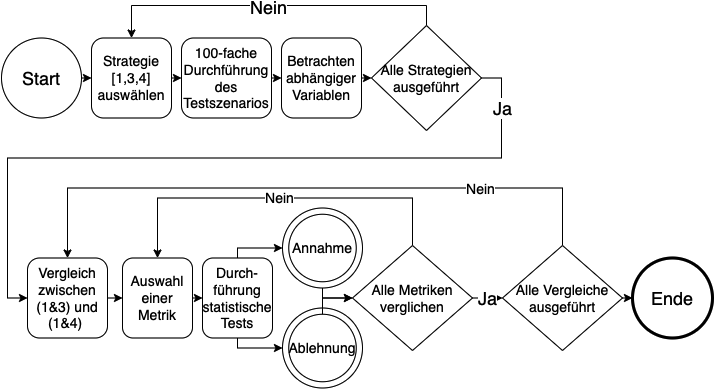
\includegraphics[height=6cm]{lib/graphics/experimentflow.png}
    \caption[BPMN Prozess des Laborexperiments]{BPMN Prozess des Laborexperiments\footnotemark}
    \label{abb:experiment flow}
\end{figure}
\footnotetext{Eigene Darstellung}